\documentclass[9pt]{extarticle}
\usepackage{core_attempt_forms}

\newcommand{\vennworkspace}{%
\begin{tikzpicture}[scale=0.38]
  \draw[thick] (-2.2,-1.6) rectangle (4.0,3.3) node[above left]{$\mathfrak U$};
  \def\rad{1.3}\coordinate (A) at (0,0);\coordinate (B) at (1.8,0);\coordinate (C) at (0.9,1.4);
  \draw (A) circle (\rad);\draw (B) circle (\rad);\draw (C) circle (\rad);
  \node at ($(A)+(0,\rad+0.35)$) {$A$};\node at ($(B)+(0,\rad+0.35)$) {$B$};\node at ($(C)+(0,\rad+0.35)$) {$C$};
\end{tikzpicture}}

\begin{document}

\CoreHeader{Sets}{S01}{A--E}{\FivePartScoring}
\begin{multicols}{2}
\begin{CoreProblem}{A}{Set language}
{\scriptsize\textit{Complete every part.}\par}
Let $S=\{x\in\mathbb Z:-2\le x<3\}$ and $T=\{-2,2\}$.
\begin{enumerate}[label=(\alph*)]
  \item Write $S$ in roster notation.
  \item Decide whether $T\subseteq S$ and whether $T\in S$.
  \item List every element of $\mathcal P(T)$.
\end{enumerate}
\end{CoreProblem}
\begin{CoreProblem}{B}{Set operations}
{\scriptsize\textit{Shade the formula's region, then name it using set operations.}\par}
$(x\in A\setminus B)\lor(x\in C)$
\begin{center}\vennworkspace\end{center}
\end{CoreProblem}
\columnbreak
\begin{CoreProblem}{C}{Relations}
{\scriptsize\textit{List the relation, evaluate both quantified statements, and classify whether it is a function.}\par}
Evaluate $\forall x\,\exists!y\,((x,y)\in R)$ and
$\forall y\,\exists!x\,((x,y)\in R)$.
\begin{center}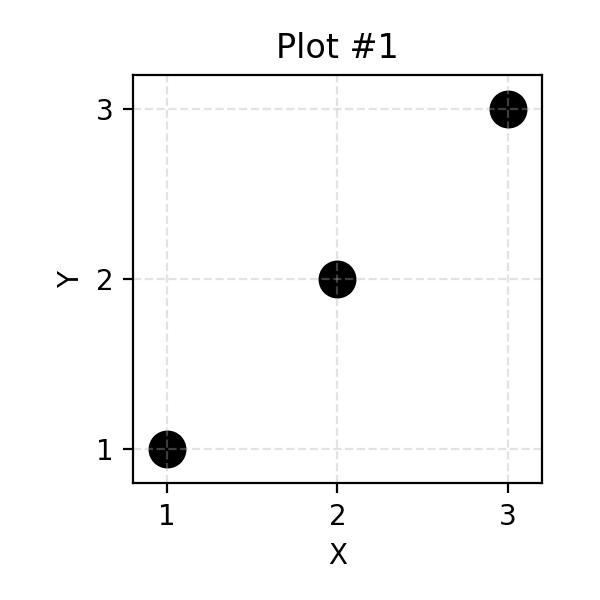
\includegraphics[width=0.52\linewidth]{../../images/set_plot1.jpg}\end{center}
\end{CoreProblem}
\begin{CoreProblem}{D}{Functions, images, and preimages}
{\scriptsize\textit{Compute the requested image/preimage and justify the function classification.}\par}
Let $A=\{1,2,3,4\}$ and $B=\{a,b,c\}$. Define $f:A\to B$ by
$f(1)=a$, $f(2)=b$, $f(3)=b$, and $f(4)=c$.
\begin{enumerate}[label=(\alph*)]
  \item Find $f(\{1,3,4\})$ and $f^{-1}(\{a,b\})$.
  \item Classify $f$ as injective, surjective, both, or neither. Justify your
  answer.
\end{enumerate}
\end{CoreProblem}
\begin{CoreProblem}{E}{Prove or refute}
{\scriptsize\textit{If true, prove by following an arbitrary element; if false, give and compute a finite counterexample.}\par}
If $f:X\to Y$ and $U,V\subseteq X$, then
\[
f(U\cup V)=f(U)\cup f(V).
\]
\end{CoreProblem}
\end{multicols}
\CoreWorkArea
\FormBreak
\CoreHeader{Sets}{S02}{A--E}{\FivePartScoring}
\begin{multicols}{2}
\begin{CoreProblem}{A}{Set language}
{\scriptsize\textit{Complete every part.}\par}
Let $S=\{x\in\mathbb Z:-4\le x\le4\text{ and }x\text{ is even}\}$ and
$T=\{-2,4\}$.
\begin{enumerate}[label=(\alph*)]
  \item Write $S$ in roster notation.
  \item Decide whether $T\subseteq S$ and whether $-2\in T$.
  \item List $T\times\{0,1\}$.
\end{enumerate}
\end{CoreProblem}
\begin{CoreProblem}{B}{Set operations}
{\scriptsize\textit{Shade the formula's region, then name it using set operations.}\par}
$(x\in \overline A)\lor(x\in B\cup C)$
\begin{center}\vennworkspace\end{center}
\end{CoreProblem}
\columnbreak
\begin{CoreProblem}{C}{Relations}
{\scriptsize\textit{List the relation, evaluate both quantified statements, and classify whether it is a function.}\par}
Evaluate $\forall x\,\exists y\,((x,y)\in R)$ and
$\exists x\,\forall y\,((x,y)\in R)$.
\begin{center}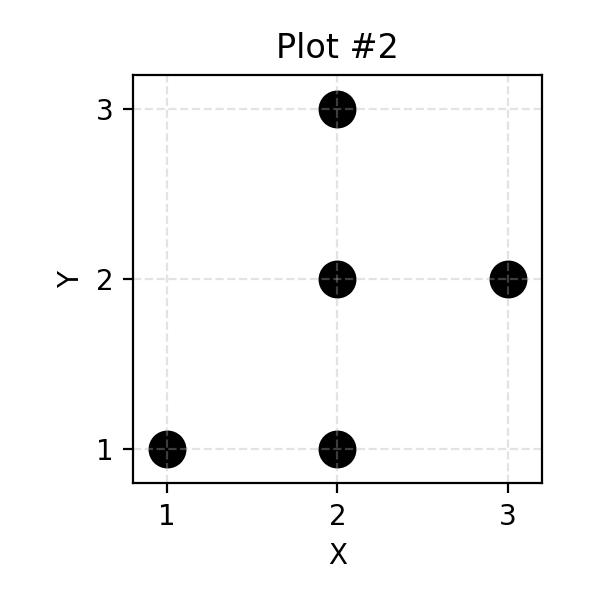
\includegraphics[width=0.52\linewidth]{../../images/set_plot2.jpg}\end{center}
\end{CoreProblem}
\begin{CoreProblem}{D}{Functions, images, and preimages}
{\scriptsize\textit{Compute the requested image/preimage and justify the function classification.}\par}
Let $g:\mathbb Z\to\mathbb Z$ be $g(n)=n+5$.
\begin{enumerate}[label=(\alph*)]
  \item Find $g(\{-1,0,2\})$ and $g^{-1}(\{4,7\})$.
  \item Classify $g$ as injective, surjective, both, or neither. Justify both
  properties.
\end{enumerate}
\end{CoreProblem}
\begin{CoreProblem}{E}{Prove or refute}
{\scriptsize\textit{If true, prove by following an arbitrary element; if false, give and compute a finite counterexample.}\par}
If $f:X\to Y$ and $U,V\subseteq X$, then
\[
f(U\cap V)=f(U)\cap f(V).
\]
\end{CoreProblem}
\end{multicols}
\CoreWorkArea
\FormBreak
\CoreHeader{Sets}{S03}{A--E}{\FivePartScoring}
\begin{multicols}{2}
\begin{CoreProblem}{A}{Set language}
{\scriptsize\textit{Complete every part.}\par}
Let $S=\{x\in\mathbb Z^+:x\mid12\}$ and $T=\{2,3\}$.
\begin{enumerate}[label=(\alph*)]
  \item Write $S$ in roster notation.
  \item Decide whether $T\subseteq S$ and whether $T\in\mathcal P(S)$.
  \item List every element of $\mathcal P(T)$.
\end{enumerate}
\end{CoreProblem}
\begin{CoreProblem}{B}{Set operations}
{\scriptsize\textit{Shade the formula's region, then name it using set operations.}\par}
$(x\in A\cup B)\to(x\in C)$
\begin{center}\vennworkspace\end{center}
\end{CoreProblem}
\columnbreak
\begin{CoreProblem}{C}{Relations}
{\scriptsize\textit{List the relation, evaluate both quantified statements, and classify whether it is a function.}\par}
Evaluate $\forall y\,\exists x\,((x,y)\in R)$ and
$\exists y\,\forall x\,((x,y)\in R)$.
\begin{center}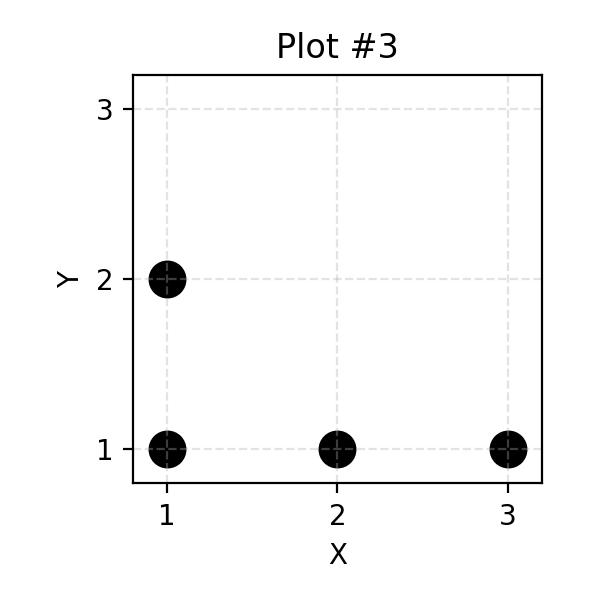
\includegraphics[width=0.52\linewidth]{../../images/set_plot3.jpg}\end{center}
\end{CoreProblem}
\begin{CoreProblem}{D}{Functions, images, and preimages}
{\scriptsize\textit{Compute the requested image/preimage and justify the function classification.}\par}
Let $h:\mathbb Z\to\mathbb Z$ be $h(n)=n^2$.
\begin{enumerate}[label=(\alph*)]
  \item Find $h(\{-2,-1,0,2\})$ and $h^{-1}(\{0,1,4\})$.
  \item Classify $h$ as injective, surjective, both, or neither. Give concrete
  witnesses for any failed property.
\end{enumerate}
\end{CoreProblem}
\begin{CoreProblem}{E}{Prove or refute}
{\scriptsize\textit{If true, prove by following an arbitrary element; if false, give and compute a finite counterexample.}\par}
If $f:X\to Y$ and $P,Q\subseteq Y$, then
\[
f^{-1}(P\cap Q)=f^{-1}(P)\cap f^{-1}(Q).
\]
\end{CoreProblem}
\end{multicols}
\CoreWorkArea
\FormBreak
\CoreHeader{Sets}{S04}{A--E}{\FivePartScoring}
\begin{multicols}{2}
\begin{CoreProblem}{A}{Set language}
{\scriptsize\textit{Complete every part.}\par}
Let $S=\{n^2:n\in\mathbb Z,-2\le n\le2\}$ and $T=\{0,1\}$.
\begin{enumerate}[label=(\alph*)]
  \item Write $S$ in roster notation, without repetitions.
  \item Decide whether $T\subset S$ and whether $2\in S$.
  \item List $T\times S$.
\end{enumerate}
\end{CoreProblem}
\begin{CoreProblem}{B}{Set operations}
{\scriptsize\textit{Shade the formula's region, then name it using set operations.}\par}
$((x\in A)\to(x\in B))\land(x\in C)$
\begin{center}\vennworkspace\end{center}
\end{CoreProblem}
\columnbreak
\begin{CoreProblem}{C}{Relations}
{\scriptsize\textit{List the relation, evaluate both quantified statements, and classify whether it is a function.}\par}
Evaluate $\forall x\,\exists!y\,((x,y)\in R)$ and
$\exists x\,\forall y\,((x,y)\in R)$.
\begin{center}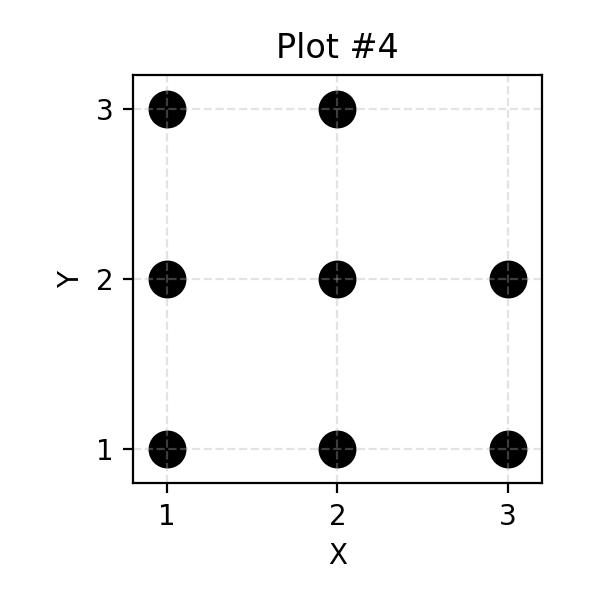
\includegraphics[width=0.52\linewidth]{../../images/set_plot4.jpg}\end{center}
\end{CoreProblem}
\begin{CoreProblem}{D}{Functions, images, and preimages}
{\scriptsize\textit{Compute the requested image/preimage and justify the function classification.}\par}
Let $k:\mathbb Z\to\mathbb Z$ be $k(n)=2n$.
\begin{enumerate}[label=(\alph*)]
  \item Find $k(\{-1,0,1\})$ and $k^{-1}(\{-2,0,4\})$.
  \item Classify $k$ as injective, surjective, both, or neither. Justify your
  answer.
\end{enumerate}
\end{CoreProblem}
\begin{CoreProblem}{E}{Prove or refute}
{\scriptsize\textit{If true, prove by following an arbitrary element; if false, give and compute a finite counterexample.}\par}
For all sets $A,B,C$,
\[
(A\cup B)\times C=(A\times C)\cup(B\times C).
\]
\end{CoreProblem}
\end{multicols}
\CoreWorkArea
\FormBreak
\CoreHeader{Sets}{S05}{A--E}{\FivePartScoring}
\begin{multicols}{2}
\begin{CoreProblem}{A}{Set language}
{\scriptsize\textit{Complete every part.}\par}
Let $S=\{x\in\mathbb Z:|x|\le2\}$ and $T=\{-1,1\}$.
\begin{enumerate}[label=(\alph*)]
  \item Write $S$ in roster notation.
  \item Decide whether $T\subseteq S$ and whether $\{0\}\in S$.
  \item List every element of $\mathcal P(T)$.
\end{enumerate}
\end{CoreProblem}
\begin{CoreProblem}{B}{Set operations}
{\scriptsize\textit{Shade the formula's region, then name it using set operations.}\par}
$(x\in A)\leftrightarrow(x\in B\setminus C)$
\begin{center}\vennworkspace\end{center}
\end{CoreProblem}
\columnbreak
\begin{CoreProblem}{C}{Relations}
{\scriptsize\textit{List the relation, evaluate both quantified statements, and classify whether it is a function.}\par}
Evaluate $\forall y\,\exists!x\,((x,y)\in R)$ and
$\exists y\,\forall x\,((x,y)\in R)$.
\begin{center}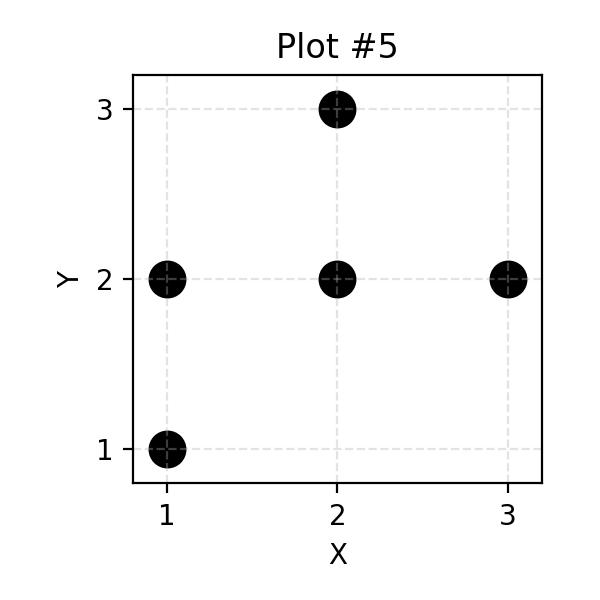
\includegraphics[width=0.52\linewidth]{../../images/set_plot5.jpg}\end{center}
\end{CoreProblem}
\begin{CoreProblem}{D}{Functions, images, and preimages}
{\scriptsize\textit{Compute the requested image/preimage and justify the function classification.}\par}
Let $q:\mathbb N_0\to\{m^2:m\in\mathbb N_0\}$ be $q(n)=n^2$, where
$\mathbb N_0=\{0,1,2,\ldots\}$.
\begin{enumerate}[label=(\alph*)]
  \item Find $q(\{0,2,3\})$ and $q^{-1}(\{1,16\})$.
  \item Classify $q$ as injective, surjective, both, or neither. Explain how
  the declared domain and codomain affect the answer.
\end{enumerate}
\end{CoreProblem}
\begin{CoreProblem}{E}{Prove or refute}
{\scriptsize\textit{If true, prove by following an arbitrary element; if false, give and compute a finite counterexample.}\par}
For all sets $A,B,C$, if $A\cup B=A\cup C$, then $B=C$.
\end{CoreProblem}
\end{multicols}
\CoreWorkArea
\FormBreak
\CoreHeader{Sets}{S06}{A--E}{\FivePartScoring}
\begin{multicols}{2}
\begin{CoreProblem}{A}{Set language}
{\scriptsize\textit{Complete every part.}\par}
Let $S=\{x\in\mathbb Z:-2\le x<3\}$ and $T=\{-2,2\}$.
\begin{enumerate}[label=(\alph*)]
  \item Write $S$ in roster notation.
  \item Decide whether $T\subseteq S$ and whether $T\in S$.
  \item List every element of $\mathcal P(T)$.
\end{enumerate}
\end{CoreProblem}
\begin{CoreProblem}{B}{Set operations}
{\scriptsize\textit{Shade the formula's region, then name it using set operations.}\par}
$(x\in \overline A)\lor(x\in B\cup C)$
\begin{center}\vennworkspace\end{center}
\end{CoreProblem}
\columnbreak
\begin{CoreProblem}{C}{Relations}
{\scriptsize\textit{List the relation, evaluate both quantified statements, and classify whether it is a function.}\par}
Evaluate $\forall y\,\exists x\,((x,y)\in R)$ and
$\exists y\,\forall x\,((x,y)\in R)$.
\begin{center}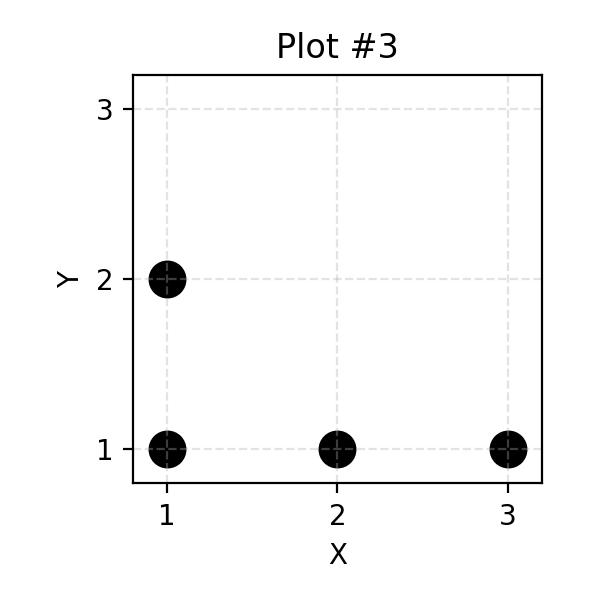
\includegraphics[width=0.52\linewidth]{../../images/set_plot3.jpg}\end{center}
\end{CoreProblem}
\begin{CoreProblem}{D}{Functions, images, and preimages}
{\scriptsize\textit{Compute the requested image/preimage and justify the function classification.}\par}
Let $k:\mathbb Z\to\mathbb Z$ be $k(n)=2n$.
\begin{enumerate}[label=(\alph*)]
  \item Find $k(\{-1,0,1\})$ and $k^{-1}(\{-2,0,4\})$.
  \item Classify $k$ as injective, surjective, both, or neither. Justify your
  answer.
\end{enumerate}
\end{CoreProblem}
\begin{CoreProblem}{E}{Prove or refute}
{\scriptsize\textit{If true, prove by following an arbitrary element; if false, give and compute a finite counterexample.}\par}
For all sets $A,B,C$, if $A\cup B=A\cup C$, then $B=C$.
\end{CoreProblem}
\end{multicols}
\CoreWorkArea
\FormBreak
\CoreHeader{Sets}{S07}{A--E}{\FivePartScoring}
\begin{multicols}{2}
\begin{CoreProblem}{A}{Set language}
{\scriptsize\textit{Complete every part.}\par}
Let $S=\{x\in\mathbb Z:-4\le x\le4\text{ and }x\text{ is even}\}$ and
$T=\{-2,4\}$.
\begin{enumerate}[label=(\alph*)]
  \item Write $S$ in roster notation.
  \item Decide whether $T\subseteq S$ and whether $-2\in T$.
  \item List $T\times\{0,1\}$.
\end{enumerate}
\end{CoreProblem}
\begin{CoreProblem}{B}{Set operations}
{\scriptsize\textit{Shade the formula's region, then name it using set operations.}\par}
$(x\in A\cup B)\to(x\in C)$
\begin{center}\vennworkspace\end{center}
\end{CoreProblem}
\columnbreak
\begin{CoreProblem}{C}{Relations}
{\scriptsize\textit{List the relation, evaluate both quantified statements, and classify whether it is a function.}\par}
Evaluate $\forall x\,\exists!y\,((x,y)\in R)$ and
$\exists x\,\forall y\,((x,y)\in R)$.
\begin{center}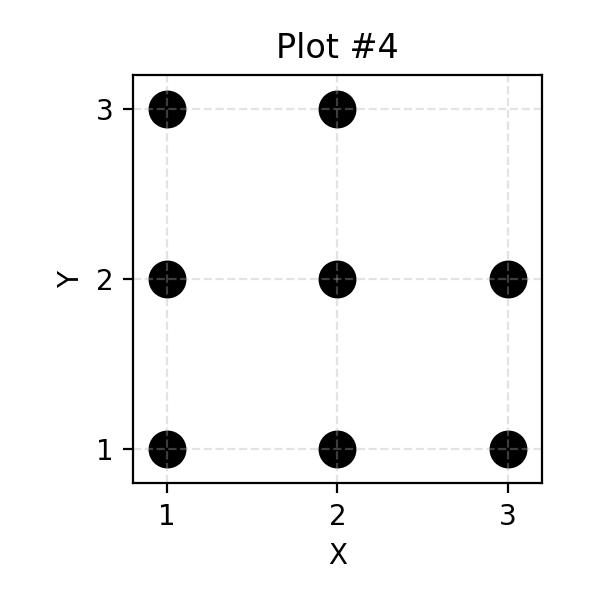
\includegraphics[width=0.52\linewidth]{../../images/set_plot4.jpg}\end{center}
\end{CoreProblem}
\begin{CoreProblem}{D}{Functions, images, and preimages}
{\scriptsize\textit{Compute the requested image/preimage and justify the function classification.}\par}
Let $q:\mathbb N_0\to\{m^2:m\in\mathbb N_0\}$ be $q(n)=n^2$, where
$\mathbb N_0=\{0,1,2,\ldots\}$.
\begin{enumerate}[label=(\alph*)]
  \item Find $q(\{0,2,3\})$ and $q^{-1}(\{1,16\})$.
  \item Classify $q$ as injective, surjective, both, or neither. Explain how
  the declared domain and codomain affect the answer.
\end{enumerate}
\end{CoreProblem}
\begin{CoreProblem}{E}{Prove or refute}
{\scriptsize\textit{If true, prove by following an arbitrary element; if false, give and compute a finite counterexample.}\par}
If $f:X\to Y$ and $U,V\subseteq X$, then
\[
f(U\cup V)=f(U)\cup f(V).
\]
\end{CoreProblem}
\end{multicols}
\CoreWorkArea
\FormBreak
\CoreHeader{Sets}{S08}{A--E}{\FivePartScoring}
\begin{multicols}{2}
\begin{CoreProblem}{A}{Set language}
{\scriptsize\textit{Complete every part.}\par}
Let $S=\{x\in\mathbb Z^+:x\mid12\}$ and $T=\{2,3\}$.
\begin{enumerate}[label=(\alph*)]
  \item Write $S$ in roster notation.
  \item Decide whether $T\subseteq S$ and whether $T\in\mathcal P(S)$.
  \item List every element of $\mathcal P(T)$.
\end{enumerate}
\end{CoreProblem}
\begin{CoreProblem}{B}{Set operations}
{\scriptsize\textit{Shade the formula's region, then name it using set operations.}\par}
$((x\in A)\to(x\in B))\land(x\in C)$
\begin{center}\vennworkspace\end{center}
\end{CoreProblem}
\columnbreak
\begin{CoreProblem}{C}{Relations}
{\scriptsize\textit{List the relation, evaluate both quantified statements, and classify whether it is a function.}\par}
Evaluate $\forall y\,\exists!x\,((x,y)\in R)$ and
$\exists y\,\forall x\,((x,y)\in R)$.
\begin{center}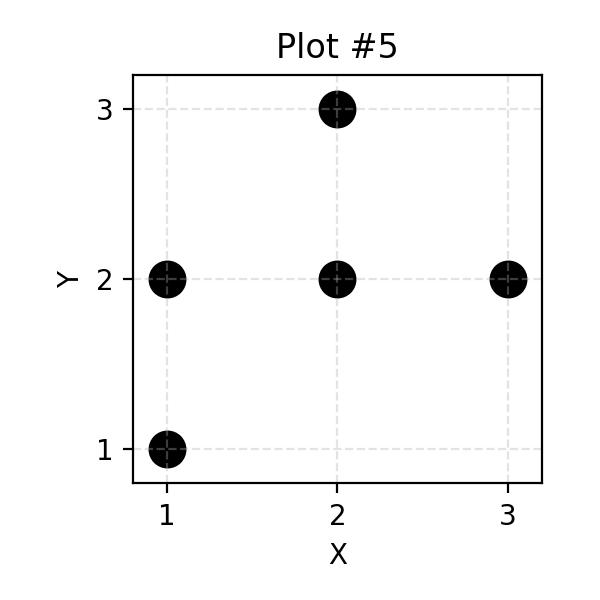
\includegraphics[width=0.52\linewidth]{../../images/set_plot5.jpg}\end{center}
\end{CoreProblem}
\begin{CoreProblem}{D}{Functions, images, and preimages}
{\scriptsize\textit{Compute the requested image/preimage and justify the function classification.}\par}
Let $A=\{1,2,3,4\}$ and $B=\{a,b,c\}$. Define $f:A\to B$ by
$f(1)=a$, $f(2)=b$, $f(3)=b$, and $f(4)=c$.
\begin{enumerate}[label=(\alph*)]
  \item Find $f(\{1,3,4\})$ and $f^{-1}(\{a,b\})$.
  \item Classify $f$ as injective, surjective, both, or neither. Justify your
  answer.
\end{enumerate}
\end{CoreProblem}
\begin{CoreProblem}{E}{Prove or refute}
{\scriptsize\textit{If true, prove by following an arbitrary element; if false, give and compute a finite counterexample.}\par}
If $f:X\to Y$ and $U,V\subseteq X$, then
\[
f(U\cap V)=f(U)\cap f(V).
\]
\end{CoreProblem}
\end{multicols}
\CoreWorkArea
\FormBreak
\CoreHeader{Sets}{S09}{A--E}{\FivePartScoring}
\begin{multicols}{2}
\begin{CoreProblem}{A}{Set language}
{\scriptsize\textit{Complete every part.}\par}
Let $S=\{n^2:n\in\mathbb Z,-2\le n\le2\}$ and $T=\{0,1\}$.
\begin{enumerate}[label=(\alph*)]
  \item Write $S$ in roster notation, without repetitions.
  \item Decide whether $T\subset S$ and whether $2\in S$.
  \item List $T\times S$.
\end{enumerate}
\end{CoreProblem}
\begin{CoreProblem}{B}{Set operations}
{\scriptsize\textit{Shade the formula's region, then name it using set operations.}\par}
$(x\in A)\leftrightarrow(x\in B\setminus C)$
\begin{center}\vennworkspace\end{center}
\end{CoreProblem}
\columnbreak
\begin{CoreProblem}{C}{Relations}
{\scriptsize\textit{List the relation, evaluate both quantified statements, and classify whether it is a function.}\par}
Evaluate $\forall x\,\exists!y\,((x,y)\in R)$ and
$\forall y\,\exists!x\,((x,y)\in R)$.
\begin{center}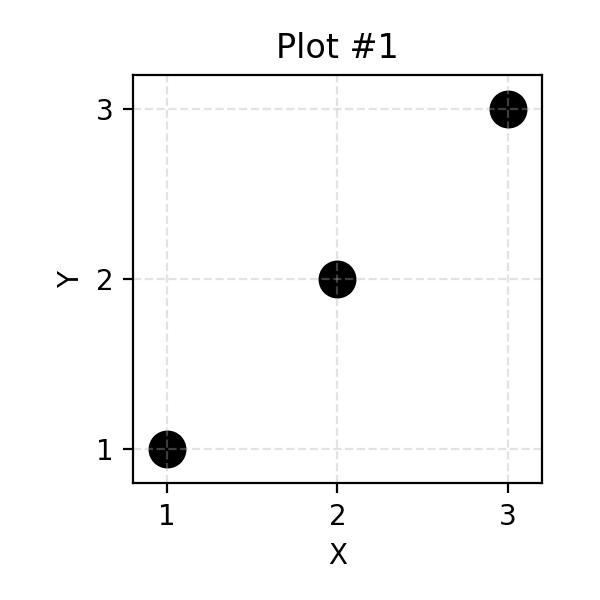
\includegraphics[width=0.52\linewidth]{../../images/set_plot1.jpg}\end{center}
\end{CoreProblem}
\begin{CoreProblem}{D}{Functions, images, and preimages}
{\scriptsize\textit{Compute the requested image/preimage and justify the function classification.}\par}
Let $g:\mathbb Z\to\mathbb Z$ be $g(n)=n+5$.
\begin{enumerate}[label=(\alph*)]
  \item Find $g(\{-1,0,2\})$ and $g^{-1}(\{4,7\})$.
  \item Classify $g$ as injective, surjective, both, or neither. Justify both
  properties.
\end{enumerate}
\end{CoreProblem}
\begin{CoreProblem}{E}{Prove or refute}
{\scriptsize\textit{If true, prove by following an arbitrary element; if false, give and compute a finite counterexample.}\par}
If $f:X\to Y$ and $P,Q\subseteq Y$, then
\[
f^{-1}(P\cap Q)=f^{-1}(P)\cap f^{-1}(Q).
\]
\end{CoreProblem}
\end{multicols}
\CoreWorkArea
\FormBreak
\CoreHeader{Sets}{S10}{A--E}{\FivePartScoring}
\begin{multicols}{2}
\begin{CoreProblem}{A}{Set language}
{\scriptsize\textit{Complete every part.}\par}
Let $S=\{x\in\mathbb Z:|x|\le2\}$ and $T=\{-1,1\}$.
\begin{enumerate}[label=(\alph*)]
  \item Write $S$ in roster notation.
  \item Decide whether $T\subseteq S$ and whether $\{0\}\in S$.
  \item List every element of $\mathcal P(T)$.
\end{enumerate}
\end{CoreProblem}
\begin{CoreProblem}{B}{Set operations}
{\scriptsize\textit{Shade the formula's region, then name it using set operations.}\par}
$(x\in A\setminus B)\lor(x\in C)$
\begin{center}\vennworkspace\end{center}
\end{CoreProblem}
\columnbreak
\begin{CoreProblem}{C}{Relations}
{\scriptsize\textit{List the relation, evaluate both quantified statements, and classify whether it is a function.}\par}
Evaluate $\forall x\,\exists y\,((x,y)\in R)$ and
$\exists x\,\forall y\,((x,y)\in R)$.
\begin{center}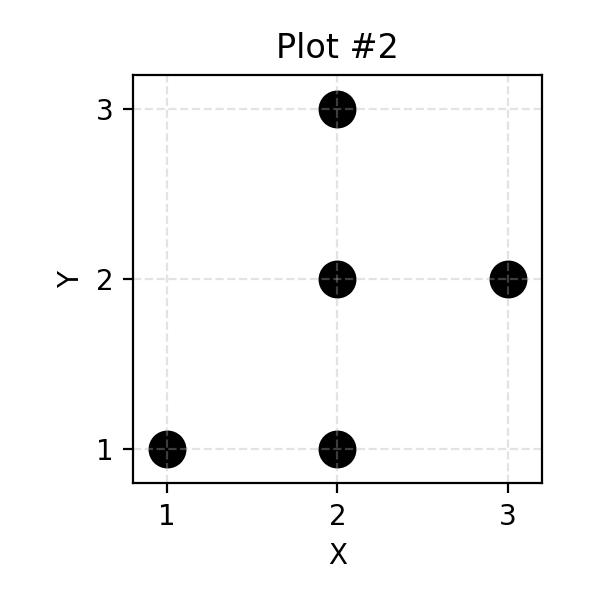
\includegraphics[width=0.52\linewidth]{../../images/set_plot2.jpg}\end{center}
\end{CoreProblem}
\begin{CoreProblem}{D}{Functions, images, and preimages}
{\scriptsize\textit{Compute the requested image/preimage and justify the function classification.}\par}
Let $h:\mathbb Z\to\mathbb Z$ be $h(n)=n^2$.
\begin{enumerate}[label=(\alph*)]
  \item Find $h(\{-2,-1,0,2\})$ and $h^{-1}(\{0,1,4\})$.
  \item Classify $h$ as injective, surjective, both, or neither. Give concrete
  witnesses for any failed property.
\end{enumerate}
\end{CoreProblem}
\begin{CoreProblem}{E}{Prove or refute}
{\scriptsize\textit{If true, prove by following an arbitrary element; if false, give and compute a finite counterexample.}\par}
For all sets $A,B,C$,
\[
(A\cup B)\times C=(A\times C)\cup(B\times C).
\]
\end{CoreProblem}
\end{multicols}
\CoreWorkArea
\FormBreak
\CoreHeader{Sets}{S11}{A--E}{\FivePartScoring}
\begin{multicols}{2}
\begin{CoreProblem}{A}{Set language}
{\scriptsize\textit{Complete every part.}\par}
Let $S=\{x\in\mathbb Z:-2\le x<3\}$ and $T=\{-2,2\}$.
\begin{enumerate}[label=(\alph*)]
  \item Write $S$ in roster notation.
  \item Decide whether $T\subseteq S$ and whether $T\in S$.
  \item List every element of $\mathcal P(T)$.
\end{enumerate}
\end{CoreProblem}
\begin{CoreProblem}{B}{Set operations}
{\scriptsize\textit{Shade the formula's region, then name it using set operations.}\par}
$(x\in A\cup B)\to(x\in C)$
\begin{center}\vennworkspace\end{center}
\end{CoreProblem}
\columnbreak
\begin{CoreProblem}{C}{Relations}
{\scriptsize\textit{List the relation, evaluate both quantified statements, and classify whether it is a function.}\par}
Evaluate $\forall y\,\exists!x\,((x,y)\in R)$ and
$\exists y\,\forall x\,((x,y)\in R)$.
\begin{center}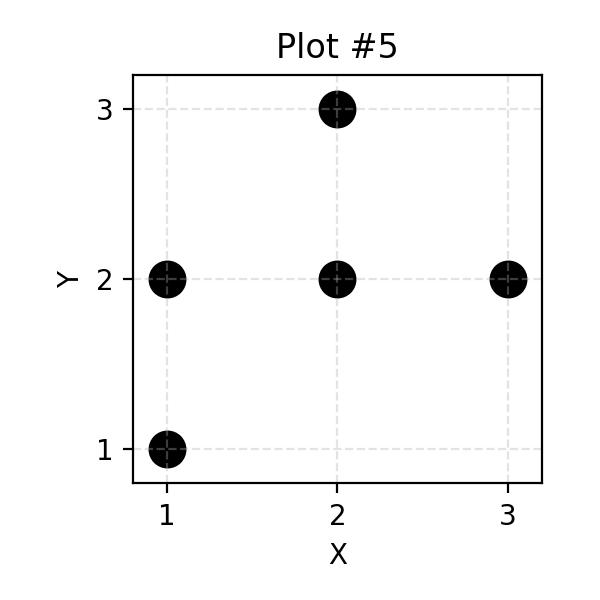
\includegraphics[width=0.52\linewidth]{../../images/set_plot5.jpg}\end{center}
\end{CoreProblem}
\begin{CoreProblem}{D}{Functions, images, and preimages}
{\scriptsize\textit{Compute the requested image/preimage and justify the function classification.}\par}
Let $g:\mathbb Z\to\mathbb Z$ be $g(n)=n+5$.
\begin{enumerate}[label=(\alph*)]
  \item Find $g(\{-1,0,2\})$ and $g^{-1}(\{4,7\})$.
  \item Classify $g$ as injective, surjective, both, or neither. Justify both
  properties.
\end{enumerate}
\end{CoreProblem}
\begin{CoreProblem}{E}{Prove or refute}
{\scriptsize\textit{If true, prove by following an arbitrary element; if false, give and compute a finite counterexample.}\par}
For all sets $A,B,C$,
\[
(A\cup B)\times C=(A\times C)\cup(B\times C).
\]
\end{CoreProblem}
\end{multicols}
\CoreWorkArea
\FormBreak
\CoreHeader{Sets}{S12}{A--E}{\FivePartScoring}
\begin{multicols}{2}
\begin{CoreProblem}{A}{Set language}
{\scriptsize\textit{Complete every part.}\par}
Let $S=\{x\in\mathbb Z:-4\le x\le4\text{ and }x\text{ is even}\}$ and
$T=\{-2,4\}$.
\begin{enumerate}[label=(\alph*)]
  \item Write $S$ in roster notation.
  \item Decide whether $T\subseteq S$ and whether $-2\in T$.
  \item List $T\times\{0,1\}$.
\end{enumerate}
\end{CoreProblem}
\begin{CoreProblem}{B}{Set operations}
{\scriptsize\textit{Shade the formula's region, then name it using set operations.}\par}
$((x\in A)\to(x\in B))\land(x\in C)$
\begin{center}\vennworkspace\end{center}
\end{CoreProblem}
\columnbreak
\begin{CoreProblem}{C}{Relations}
{\scriptsize\textit{List the relation, evaluate both quantified statements, and classify whether it is a function.}\par}
Evaluate $\forall x\,\exists!y\,((x,y)\in R)$ and
$\forall y\,\exists!x\,((x,y)\in R)$.
\begin{center}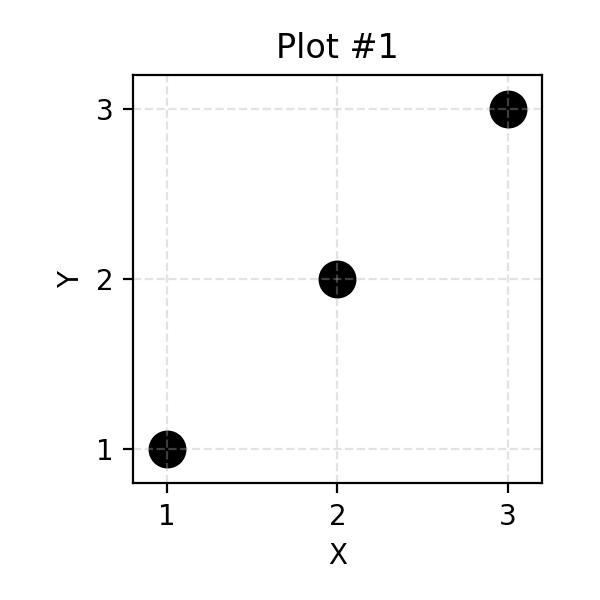
\includegraphics[width=0.52\linewidth]{../../images/set_plot1.jpg}\end{center}
\end{CoreProblem}
\begin{CoreProblem}{D}{Functions, images, and preimages}
{\scriptsize\textit{Compute the requested image/preimage and justify the function classification.}\par}
Let $h:\mathbb Z\to\mathbb Z$ be $h(n)=n^2$.
\begin{enumerate}[label=(\alph*)]
  \item Find $h(\{-2,-1,0,2\})$ and $h^{-1}(\{0,1,4\})$.
  \item Classify $h$ as injective, surjective, both, or neither. Give concrete
  witnesses for any failed property.
\end{enumerate}
\end{CoreProblem}
\begin{CoreProblem}{E}{Prove or refute}
{\scriptsize\textit{If true, prove by following an arbitrary element; if false, give and compute a finite counterexample.}\par}
For all sets $A,B,C$, if $A\cup B=A\cup C$, then $B=C$.
\end{CoreProblem}
\end{multicols}
\CoreWorkArea
\FormBreak
\CoreHeader{Sets}{S13}{A--E}{\FivePartScoring}
\begin{multicols}{2}
\begin{CoreProblem}{A}{Set language}
{\scriptsize\textit{Complete every part.}\par}
Let $S=\{x\in\mathbb Z^+:x\mid12\}$ and $T=\{2,3\}$.
\begin{enumerate}[label=(\alph*)]
  \item Write $S$ in roster notation.
  \item Decide whether $T\subseteq S$ and whether $T\in\mathcal P(S)$.
  \item List every element of $\mathcal P(T)$.
\end{enumerate}
\end{CoreProblem}
\begin{CoreProblem}{B}{Set operations}
{\scriptsize\textit{Shade the formula's region, then name it using set operations.}\par}
$(x\in A)\leftrightarrow(x\in B\setminus C)$
\begin{center}\vennworkspace\end{center}
\end{CoreProblem}
\columnbreak
\begin{CoreProblem}{C}{Relations}
{\scriptsize\textit{List the relation, evaluate both quantified statements, and classify whether it is a function.}\par}
Evaluate $\forall x\,\exists y\,((x,y)\in R)$ and
$\exists x\,\forall y\,((x,y)\in R)$.
\begin{center}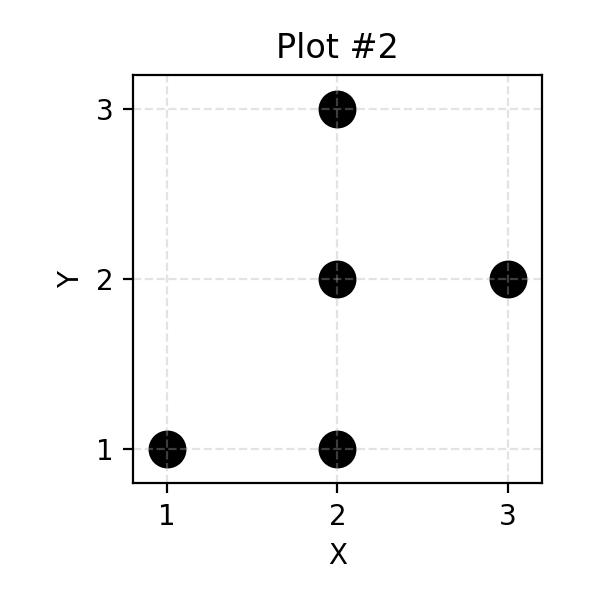
\includegraphics[width=0.52\linewidth]{../../images/set_plot2.jpg}\end{center}
\end{CoreProblem}
\begin{CoreProblem}{D}{Functions, images, and preimages}
{\scriptsize\textit{Compute the requested image/preimage and justify the function classification.}\par}
Let $k:\mathbb Z\to\mathbb Z$ be $k(n)=2n$.
\begin{enumerate}[label=(\alph*)]
  \item Find $k(\{-1,0,1\})$ and $k^{-1}(\{-2,0,4\})$.
  \item Classify $k$ as injective, surjective, both, or neither. Justify your
  answer.
\end{enumerate}
\end{CoreProblem}
\begin{CoreProblem}{E}{Prove or refute}
{\scriptsize\textit{If true, prove by following an arbitrary element; if false, give and compute a finite counterexample.}\par}
If $f:X\to Y$ and $U,V\subseteq X$, then
\[
f(U\cup V)=f(U)\cup f(V).
\]
\end{CoreProblem}
\end{multicols}
\CoreWorkArea
\FormBreak
\CoreHeader{Sets}{S14}{A--E}{\FivePartScoring}
\begin{multicols}{2}
\begin{CoreProblem}{A}{Set language}
{\scriptsize\textit{Complete every part.}\par}
Let $S=\{n^2:n\in\mathbb Z,-2\le n\le2\}$ and $T=\{0,1\}$.
\begin{enumerate}[label=(\alph*)]
  \item Write $S$ in roster notation, without repetitions.
  \item Decide whether $T\subset S$ and whether $2\in S$.
  \item List $T\times S$.
\end{enumerate}
\end{CoreProblem}
\begin{CoreProblem}{B}{Set operations}
{\scriptsize\textit{Shade the formula's region, then name it using set operations.}\par}
$(x\in A\setminus B)\lor(x\in C)$
\begin{center}\vennworkspace\end{center}
\end{CoreProblem}
\columnbreak
\begin{CoreProblem}{C}{Relations}
{\scriptsize\textit{List the relation, evaluate both quantified statements, and classify whether it is a function.}\par}
Evaluate $\forall y\,\exists x\,((x,y)\in R)$ and
$\exists y\,\forall x\,((x,y)\in R)$.
\begin{center}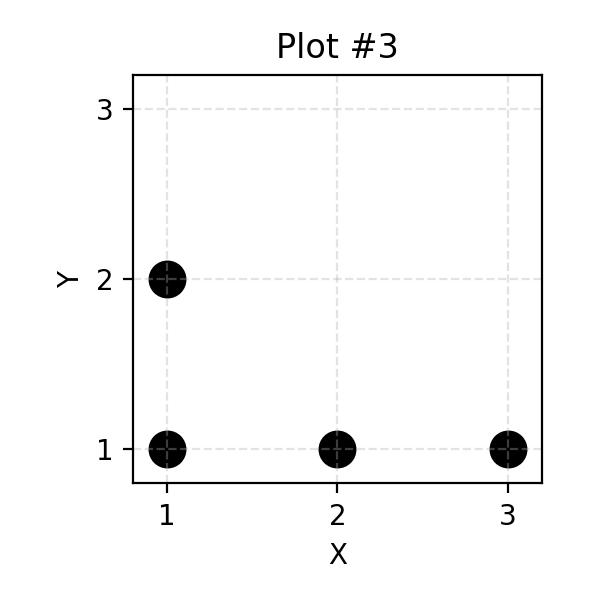
\includegraphics[width=0.52\linewidth]{../../images/set_plot3.jpg}\end{center}
\end{CoreProblem}
\begin{CoreProblem}{D}{Functions, images, and preimages}
{\scriptsize\textit{Compute the requested image/preimage and justify the function classification.}\par}
Let $q:\mathbb N_0\to\{m^2:m\in\mathbb N_0\}$ be $q(n)=n^2$, where
$\mathbb N_0=\{0,1,2,\ldots\}$.
\begin{enumerate}[label=(\alph*)]
  \item Find $q(\{0,2,3\})$ and $q^{-1}(\{1,16\})$.
  \item Classify $q$ as injective, surjective, both, or neither. Explain how
  the declared domain and codomain affect the answer.
\end{enumerate}
\end{CoreProblem}
\begin{CoreProblem}{E}{Prove or refute}
{\scriptsize\textit{If true, prove by following an arbitrary element; if false, give and compute a finite counterexample.}\par}
If $f:X\to Y$ and $U,V\subseteq X$, then
\[
f(U\cap V)=f(U)\cap f(V).
\]
\end{CoreProblem}
\end{multicols}
\CoreWorkArea
\FormBreak
\CoreHeader{Sets}{S15}{A--E}{\FivePartScoring}
\begin{multicols}{2}
\begin{CoreProblem}{A}{Set language}
{\scriptsize\textit{Complete every part.}\par}
Let $S=\{x\in\mathbb Z:|x|\le2\}$ and $T=\{-1,1\}$.
\begin{enumerate}[label=(\alph*)]
  \item Write $S$ in roster notation.
  \item Decide whether $T\subseteq S$ and whether $\{0\}\in S$.
  \item List every element of $\mathcal P(T)$.
\end{enumerate}
\end{CoreProblem}
\begin{CoreProblem}{B}{Set operations}
{\scriptsize\textit{Shade the formula's region, then name it using set operations.}\par}
$(x\in \overline A)\lor(x\in B\cup C)$
\begin{center}\vennworkspace\end{center}
\end{CoreProblem}
\columnbreak
\begin{CoreProblem}{C}{Relations}
{\scriptsize\textit{List the relation, evaluate both quantified statements, and classify whether it is a function.}\par}
Evaluate $\forall x\,\exists!y\,((x,y)\in R)$ and
$\exists x\,\forall y\,((x,y)\in R)$.
\begin{center}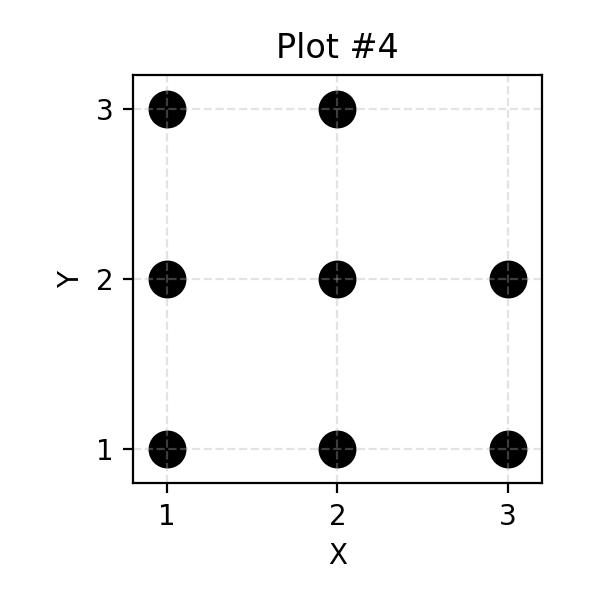
\includegraphics[width=0.52\linewidth]{../../images/set_plot4.jpg}\end{center}
\end{CoreProblem}
\begin{CoreProblem}{D}{Functions, images, and preimages}
{\scriptsize\textit{Compute the requested image/preimage and justify the function classification.}\par}
Let $A=\{1,2,3,4\}$ and $B=\{a,b,c\}$. Define $f:A\to B$ by
$f(1)=a$, $f(2)=b$, $f(3)=b$, and $f(4)=c$.
\begin{enumerate}[label=(\alph*)]
  \item Find $f(\{1,3,4\})$ and $f^{-1}(\{a,b\})$.
  \item Classify $f$ as injective, surjective, both, or neither. Justify your
  answer.
\end{enumerate}
\end{CoreProblem}
\begin{CoreProblem}{E}{Prove or refute}
{\scriptsize\textit{If true, prove by following an arbitrary element; if false, give and compute a finite counterexample.}\par}
If $f:X\to Y$ and $P,Q\subseteq Y$, then
\[
f^{-1}(P\cap Q)=f^{-1}(P)\cap f^{-1}(Q).
\]
\end{CoreProblem}
\end{multicols}
\CoreWorkArea
\FormBreak
\CoreHeader{Sets}{S16}{A--E}{\FivePartScoring}
\begin{multicols}{2}
\begin{CoreProblem}{A}{Set language}
{\scriptsize\textit{Complete every part.}\par}
Let $S=\{x\in\mathbb Z:-2\le x<3\}$ and $T=\{-2,2\}$.
\begin{enumerate}[label=(\alph*)]
  \item Write $S$ in roster notation.
  \item Decide whether $T\subseteq S$ and whether $T\in S$.
  \item List every element of $\mathcal P(T)$.
\end{enumerate}
\end{CoreProblem}
\begin{CoreProblem}{B}{Set operations}
{\scriptsize\textit{Shade the formula's region, then name it using set operations.}\par}
$((x\in A)\to(x\in B))\land(x\in C)$
\begin{center}\vennworkspace\end{center}
\end{CoreProblem}
\columnbreak
\begin{CoreProblem}{C}{Relations}
{\scriptsize\textit{List the relation, evaluate both quantified statements, and classify whether it is a function.}\par}
Evaluate $\forall x\,\exists y\,((x,y)\in R)$ and
$\exists x\,\forall y\,((x,y)\in R)$.
\begin{center}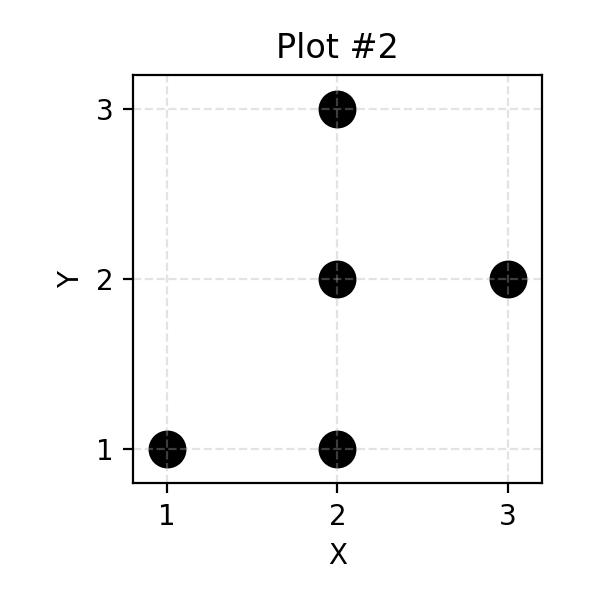
\includegraphics[width=0.52\linewidth]{../../images/set_plot2.jpg}\end{center}
\end{CoreProblem}
\begin{CoreProblem}{D}{Functions, images, and preimages}
{\scriptsize\textit{Compute the requested image/preimage and justify the function classification.}\par}
Let $q:\mathbb N_0\to\{m^2:m\in\mathbb N_0\}$ be $q(n)=n^2$, where
$\mathbb N_0=\{0,1,2,\ldots\}$.
\begin{enumerate}[label=(\alph*)]
  \item Find $q(\{0,2,3\})$ and $q^{-1}(\{1,16\})$.
  \item Classify $q$ as injective, surjective, both, or neither. Explain how
  the declared domain and codomain affect the answer.
\end{enumerate}
\end{CoreProblem}
\begin{CoreProblem}{E}{Prove or refute}
{\scriptsize\textit{If true, prove by following an arbitrary element; if false, give and compute a finite counterexample.}\par}
If $f:X\to Y$ and $P,Q\subseteq Y$, then
\[
f^{-1}(P\cap Q)=f^{-1}(P)\cap f^{-1}(Q).
\]
\end{CoreProblem}
\end{multicols}
\CoreWorkArea
\FormBreak
\CoreHeader{Sets}{S17}{A--E}{\FivePartScoring}
\begin{multicols}{2}
\begin{CoreProblem}{A}{Set language}
{\scriptsize\textit{Complete every part.}\par}
Let $S=\{x\in\mathbb Z:-4\le x\le4\text{ and }x\text{ is even}\}$ and
$T=\{-2,4\}$.
\begin{enumerate}[label=(\alph*)]
  \item Write $S$ in roster notation.
  \item Decide whether $T\subseteq S$ and whether $-2\in T$.
  \item List $T\times\{0,1\}$.
\end{enumerate}
\end{CoreProblem}
\begin{CoreProblem}{B}{Set operations}
{\scriptsize\textit{Shade the formula's region, then name it using set operations.}\par}
$(x\in A)\leftrightarrow(x\in B\setminus C)$
\begin{center}\vennworkspace\end{center}
\end{CoreProblem}
\columnbreak
\begin{CoreProblem}{C}{Relations}
{\scriptsize\textit{List the relation, evaluate both quantified statements, and classify whether it is a function.}\par}
Evaluate $\forall y\,\exists x\,((x,y)\in R)$ and
$\exists y\,\forall x\,((x,y)\in R)$.
\begin{center}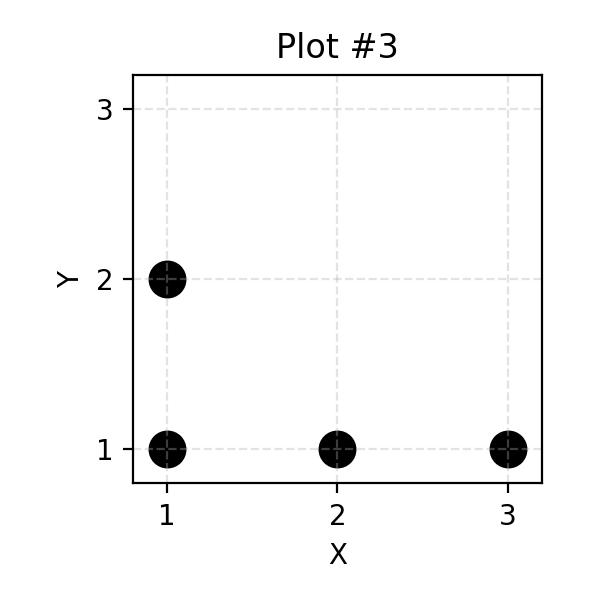
\includegraphics[width=0.52\linewidth]{../../images/set_plot3.jpg}\end{center}
\end{CoreProblem}
\begin{CoreProblem}{D}{Functions, images, and preimages}
{\scriptsize\textit{Compute the requested image/preimage and justify the function classification.}\par}
Let $A=\{1,2,3,4\}$ and $B=\{a,b,c\}$. Define $f:A\to B$ by
$f(1)=a$, $f(2)=b$, $f(3)=b$, and $f(4)=c$.
\begin{enumerate}[label=(\alph*)]
  \item Find $f(\{1,3,4\})$ and $f^{-1}(\{a,b\})$.
  \item Classify $f$ as injective, surjective, both, or neither. Justify your
  answer.
\end{enumerate}
\end{CoreProblem}
\begin{CoreProblem}{E}{Prove or refute}
{\scriptsize\textit{If true, prove by following an arbitrary element; if false, give and compute a finite counterexample.}\par}
For all sets $A,B,C$,
\[
(A\cup B)\times C=(A\times C)\cup(B\times C).
\]
\end{CoreProblem}
\end{multicols}
\CoreWorkArea
\FormBreak
\CoreHeader{Sets}{S18}{A--E}{\FivePartScoring}
\begin{multicols}{2}
\begin{CoreProblem}{A}{Set language}
{\scriptsize\textit{Complete every part.}\par}
Let $S=\{x\in\mathbb Z^+:x\mid12\}$ and $T=\{2,3\}$.
\begin{enumerate}[label=(\alph*)]
  \item Write $S$ in roster notation.
  \item Decide whether $T\subseteq S$ and whether $T\in\mathcal P(S)$.
  \item List every element of $\mathcal P(T)$.
\end{enumerate}
\end{CoreProblem}
\begin{CoreProblem}{B}{Set operations}
{\scriptsize\textit{Shade the formula's region, then name it using set operations.}\par}
$(x\in A\setminus B)\lor(x\in C)$
\begin{center}\vennworkspace\end{center}
\end{CoreProblem}
\columnbreak
\begin{CoreProblem}{C}{Relations}
{\scriptsize\textit{List the relation, evaluate both quantified statements, and classify whether it is a function.}\par}
Evaluate $\forall x\,\exists!y\,((x,y)\in R)$ and
$\exists x\,\forall y\,((x,y)\in R)$.
\begin{center}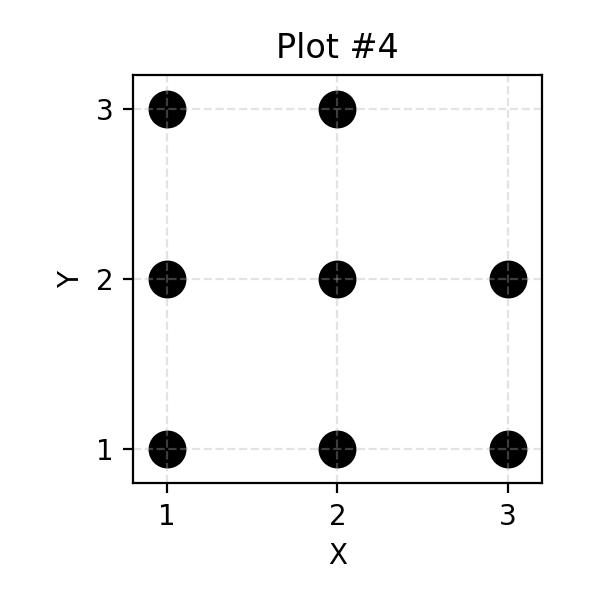
\includegraphics[width=0.52\linewidth]{../../images/set_plot4.jpg}\end{center}
\end{CoreProblem}
\begin{CoreProblem}{D}{Functions, images, and preimages}
{\scriptsize\textit{Compute the requested image/preimage and justify the function classification.}\par}
Let $g:\mathbb Z\to\mathbb Z$ be $g(n)=n+5$.
\begin{enumerate}[label=(\alph*)]
  \item Find $g(\{-1,0,2\})$ and $g^{-1}(\{4,7\})$.
  \item Classify $g$ as injective, surjective, both, or neither. Justify both
  properties.
\end{enumerate}
\end{CoreProblem}
\begin{CoreProblem}{E}{Prove or refute}
{\scriptsize\textit{If true, prove by following an arbitrary element; if false, give and compute a finite counterexample.}\par}
For all sets $A,B,C$, if $A\cup B=A\cup C$, then $B=C$.
\end{CoreProblem}
\end{multicols}
\CoreWorkArea
\FormBreak
\CoreHeader{Sets}{S19}{A--E}{\FivePartScoring}
\begin{multicols}{2}
\begin{CoreProblem}{A}{Set language}
{\scriptsize\textit{Complete every part.}\par}
Let $S=\{n^2:n\in\mathbb Z,-2\le n\le2\}$ and $T=\{0,1\}$.
\begin{enumerate}[label=(\alph*)]
  \item Write $S$ in roster notation, without repetitions.
  \item Decide whether $T\subset S$ and whether $2\in S$.
  \item List $T\times S$.
\end{enumerate}
\end{CoreProblem}
\begin{CoreProblem}{B}{Set operations}
{\scriptsize\textit{Shade the formula's region, then name it using set operations.}\par}
$(x\in \overline A)\lor(x\in B\cup C)$
\begin{center}\vennworkspace\end{center}
\end{CoreProblem}
\columnbreak
\begin{CoreProblem}{C}{Relations}
{\scriptsize\textit{List the relation, evaluate both quantified statements, and classify whether it is a function.}\par}
Evaluate $\forall y\,\exists!x\,((x,y)\in R)$ and
$\exists y\,\forall x\,((x,y)\in R)$.
\begin{center}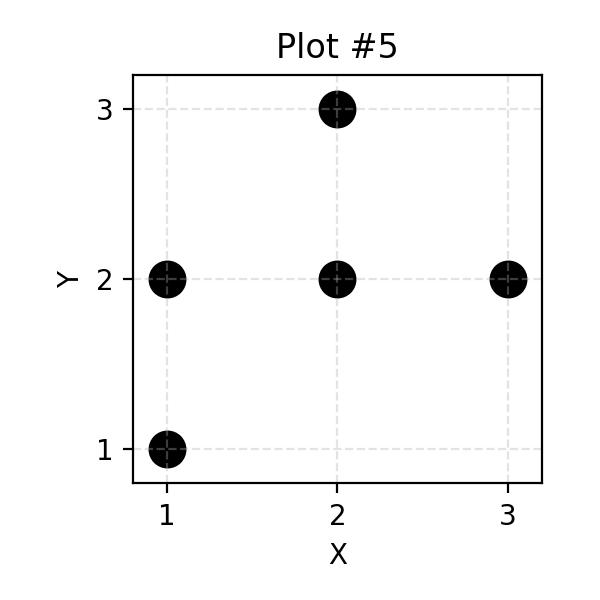
\includegraphics[width=0.52\linewidth]{../../images/set_plot5.jpg}\end{center}
\end{CoreProblem}
\begin{CoreProblem}{D}{Functions, images, and preimages}
{\scriptsize\textit{Compute the requested image/preimage and justify the function classification.}\par}
Let $h:\mathbb Z\to\mathbb Z$ be $h(n)=n^2$.
\begin{enumerate}[label=(\alph*)]
  \item Find $h(\{-2,-1,0,2\})$ and $h^{-1}(\{0,1,4\})$.
  \item Classify $h$ as injective, surjective, both, or neither. Give concrete
  witnesses for any failed property.
\end{enumerate}
\end{CoreProblem}
\begin{CoreProblem}{E}{Prove or refute}
{\scriptsize\textit{If true, prove by following an arbitrary element; if false, give and compute a finite counterexample.}\par}
If $f:X\to Y$ and $U,V\subseteq X$, then
\[
f(U\cup V)=f(U)\cup f(V).
\]
\end{CoreProblem}
\end{multicols}
\CoreWorkArea
\FormBreak
\CoreHeader{Sets}{S20}{A--E}{\FivePartScoring}
\begin{multicols}{2}
\begin{CoreProblem}{A}{Set language}
{\scriptsize\textit{Complete every part.}\par}
Let $S=\{x\in\mathbb Z:|x|\le2\}$ and $T=\{-1,1\}$.
\begin{enumerate}[label=(\alph*)]
  \item Write $S$ in roster notation.
  \item Decide whether $T\subseteq S$ and whether $\{0\}\in S$.
  \item List every element of $\mathcal P(T)$.
\end{enumerate}
\end{CoreProblem}
\begin{CoreProblem}{B}{Set operations}
{\scriptsize\textit{Shade the formula's region, then name it using set operations.}\par}
$(x\in A\cup B)\to(x\in C)$
\begin{center}\vennworkspace\end{center}
\end{CoreProblem}
\columnbreak
\begin{CoreProblem}{C}{Relations}
{\scriptsize\textit{List the relation, evaluate both quantified statements, and classify whether it is a function.}\par}
Evaluate $\forall x\,\exists!y\,((x,y)\in R)$ and
$\forall y\,\exists!x\,((x,y)\in R)$.
\begin{center}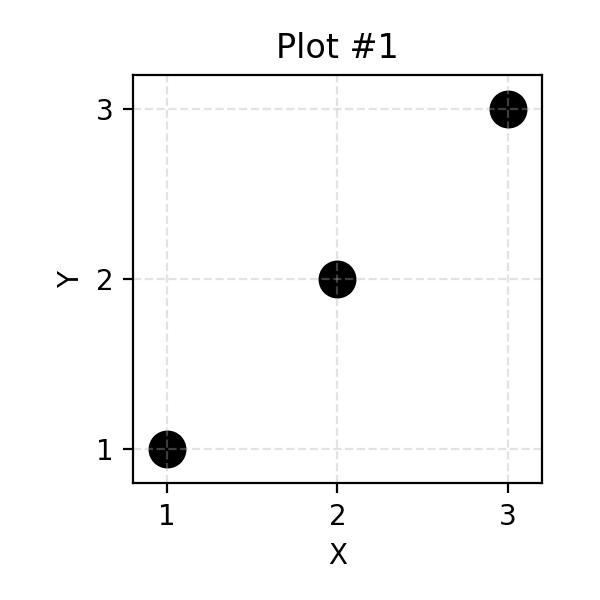
\includegraphics[width=0.52\linewidth]{../../images/set_plot1.jpg}\end{center}
\end{CoreProblem}
\begin{CoreProblem}{D}{Functions, images, and preimages}
{\scriptsize\textit{Compute the requested image/preimage and justify the function classification.}\par}
Let $k:\mathbb Z\to\mathbb Z$ be $k(n)=2n$.
\begin{enumerate}[label=(\alph*)]
  \item Find $k(\{-1,0,1\})$ and $k^{-1}(\{-2,0,4\})$.
  \item Classify $k$ as injective, surjective, both, or neither. Justify your
  answer.
\end{enumerate}
\end{CoreProblem}
\begin{CoreProblem}{E}{Prove or refute}
{\scriptsize\textit{If true, prove by following an arbitrary element; if false, give and compute a finite counterexample.}\par}
If $f:X\to Y$ and $U,V\subseteq X$, then
\[
f(U\cap V)=f(U)\cap f(V).
\]
\end{CoreProblem}
\end{multicols}
\CoreWorkArea
\end{document}
